\documentclass[russian,xcolor=dvipsnames]{beamer}
%\mode<presentation>{\usetheme{CambridgeUS}}

\mode<presentation>{\usetheme{Madrid}}

\useoutertheme{miniframes} % Alternatively: miniframes, infolines, split
\useinnertheme{circles}
% \setbeamertemplate{footline}{}

\definecolor{UBCblue}{rgb}{0.2, 0.2, 0.6} % UBC Blue (primary)
\definecolor{UBCgrey}{rgb}{1, 0.49, 0.0} % UBC Grey (secondary)

\setbeamercolor{palette primary}{bg=UBCblue,fg=white}
\setbeamercolor{palette secondary}{bg=UBCblue,fg=white}
\setbeamercolor{palette tertiary}{bg=UBCblue,fg=white}
\setbeamercolor{palette quaternary}{bg=UBCblue,fg=white}
\setbeamercolor{structure}{fg=UBCblue} % itemize, enumerate, etc
\setbeamercolor{section in toc}{fg=UBCblue} % TOC sections

% Override palette coloring with secondary
\setbeamercolor{subsection in head/foot}{bg=UBCgrey,fg=black}
% \setbeamercovered{only}

%\definecolor{UBCblue}{rgb}{0.04706, 0.13725, 0.26667} % UBC Blue (primary)
%
%\usecolortheme[named=UBCblue]{structure}

%\definecolor{UniBlue}{RGB}{83,121,170}
%\setbeamercolor{title}{fg=UniBlue}
%\setbeamercolor{frametitle}{fg=UniBlue}
%\setbeamercolor{structure}{fg=UniBlue}
%
%\definecolor{cvut_navy}{HTML}{0065BD}
%\definecolor{cvut_blue}{HTML}{6AADE4}
%\definecolor{cvut_gray}{HTML}{156570}
%
%\setbeamercolor{section in toc}{fg=black,bg=white}
%\setbeamercolor{alerted text}{fg=cvut_blue}
%\setbeamercolor*{palette primary}{bg=cvut_navy,fg=gray!20!white}
%\setbeamercolor*{palette secondary}{bg=cvut_blue,fg=white}
%\setbeamercolor*{palette tertiary}{parent=palette primary}
%\setbeamercolor*{palette quaternary}{fg=green,bg=gray!5!white}
%
%\setbeamercolor*{sidebar}{fg=cvut_navy,bg=gray!15!white}
%
%
%\setbeamercolor{titlelike}{parent=palette primary}
%\setbeamercolor{frametitle}{parent=palette primary}

\usepackage[utf8]{inputenc}
\usepackage[T1, T2A]{fontenc}
\usepackage[russian,english]{babel}
% \usepackage{cmap}
\usepackage{amsmath,amsfonts,amsthm,amssymb,amsbsy,amstext,amscd,amsxtra,multicol}
\usepackage{units}
\usepackage{fancyhdr}
\usepackage{forloop}
\usepackage{indentfirst}
\usepackage{verbatim}
\usepackage{tikz}
\usetikzlibrary{automata,positioning}
\usepackage{graphicx}
\usepackage[stable]{footmisc}
\usepackage{color}
\usepackage{pstricks}
% \usepackage{algorithmic}
\usepackage{algorithm}
\makeatletter
\renewcommand{\ALG@name}{Алгоритм}
\makeatother
\usepackage{algpseudocode}

\definecolor{col_e}{RGB}{10, 150, 50}
\definecolor{col_delzeta}{RGB}{115, 8, 8}
\definecolor{col_deleta}{RGB}{0, 0, 139}



\usepackage{url}
% \usepackage{hyperref}
%\usepackage{algorithm}
%%\usepackage{algorithmic}
%%\usepackage[algo2e]{algorithm2e}
%\usepackage{algpseudocode}
\usepackage{tabularx}
%\usepackage{paralist}
\usepackage{mathtools}
\usepackage{tcolorbox}
\usepackage{makecell}
\usepackage{wrapfig}
\usepackage{ulem}

\usepackage{pifont}
\newcommand{\cmark}{{\color{PineGreen}\ding{51}}}%
\newcommand{\xmark}{{\color{BrickRed}\ding{55}}}%

\usepackage{bibentry}
%  \usepackage{natbib}
%\usepackage{sidecap}
%\renewcommand{\bibname}{References}
%\renewcommand{\bibsection}{\subsubsection*{\bibname}}
%\bibliographystyle{abbrvnat}

\renewcommand{\algorithmicrequire}{\textbf{Вход:}}
\renewcommand{\algorithmicensure}{\textbf{Выход:}}
\usepackage{subfigure} 
\newcommand{\Exp}{\mathbf{E}}
% \newcommand{\Prob}{\mathbf{P}}
\newcommand{\R}{\mathbb{R}}

\newcommand{\eqdef}{\stackrel{\text{def}}{=}}
%\newcommand{\eqdef}{\coloneqq}

\newcommand{\ve}[2]{\left\langle #1 , #2 \right\rangle}
\def\<#1,#2>{\left\langle #1,#2\right\rangle}


\newcommand{\oldstuff}[1]{ {\small \color{blue} #1}}
\newcommand{\redstuff}[1]{ {\small \color{red} #1}}

%\theoremstyle{definition}
%\newtheorem{lemma}{Lemma}
%\newtheorem{theorem}{Theorem}
%\newtheorem{definition}{Definition}
%\newtheorem{proposition}{Proposition}
%\newtheorem{assumption}{Assumption}
%\newtheorem{corollary}{Corollary}
%\newtheorem{example}{Example}
%\theoremstyle{definition}
\newtheorem{prop}[theorem]{Proposition}
\newtheorem{ass}[theorem]{Assumption}
\newtheorem{lem}[theorem]{Lemma}
\newtheorem{thm}[theorem]{Theorem}
\newtheorem{cor}[theorem]{Corollary}
\newtheorem{remark}[theorem]{Remark}



\newcommand\tagthis{\addtocounter{equation}{1}\tag{\theequation}}
\newcommand{\argmin}{\mathop{\arg\!\min}}
\newcommand{\circledOne}{\text{\ding{172}}}
\newcommand{\circledTwo}{\text{\ding{173}}}
\newcommand{\circledThree}{\text{\ding{174}}}
\newcommand{\circledFour}{\text{\ding{175}}}
\newcommand{\circledFive}{\text{\ding{176}}}
\newcommand{\circledSix}{\text{\ding{177}}}
\newcommand{\circledSeven}{\text{\ding{178}}}
\newcommand{\circledEight}{\text{\ding{179}}}
\newcommand{\circledNine}{\text{\ding{180}}}
\newcommand{\circledTen}{\text{\ding{181}}}

% TO DO NOTES 
%\usepackage[colorinlistoftodos,bordercolor=orange,backgroundcolor=orange!20,linecolor=orange,textsize=scriptsize]{todonotes}
%
%\newcommand{\peter}[1]{\todo[inline]{{\textbf{Peter:} \emph{#1}}}}
%\newcommand{\eduard}[1]{\todo[inline]{{\textbf{Eduard:} \emph{#1}}}}
%\newcommand{\filip}[1]{\todo[inline]{{\textbf{Filip:} \emph{#1}}}}

% TO DO NOTES 
%\usepackage[colorinlistoftodos,bordercolor=orange,backgroundcolor=orange!20,linecolor=orange,textsize=scriptsize]{todonotes}
%
%\newcommand{\peter}[1]{\todo[inline]{{\textbf{Peter:} \emph{#1}}}}
%\newcommand{\eduard}[1]{\todo[inline]{{\textbf{Eduard:} \emph{#1}}}}
%\newcommand{\filip}[1]{\todo[inline]{{\textbf{Filip:} \emph{#1}}}}


% caligraphic
\newcommand{\cA}{{\cal A}}
\newcommand{\cB}{{\cal B}}
\newcommand{\cC}{{\cal C}}
\newcommand{\cD}{{\cal D}}
\newcommand{\cE}{{\cal E}}
\newcommand{\cF}{{\cal F}}
\newcommand{\cG}{{\cal G}}
\newcommand{\cH}{{\cal H}}
\newcommand{\cJ}{{\cal J}}
\newcommand{\cK}{{\cal K}}
\newcommand{\cL}{{\cal L}}
\newcommand{\cM}{{\cal M}}
\newcommand{\cN}{{\cal N}}
\newcommand{\cO}{{\cal O}}
\newcommand{\cP}{{\cal P}}
\newcommand{\cQ}{{\cal Q}}
\newcommand{\cR}{{\cal R}}
\newcommand{\cS}{{\cal S}}
\newcommand{\cT}{{\cal T}}
\newcommand{\cU}{{\cal U}}
\newcommand{\cV}{{\cal V}}
\newcommand{\cX}{{\cal X}}
\newcommand{\cY}{{\cal Y}}
\newcommand{\cW}{{\cal W}}
\newcommand{\cZ}{{\cal Z}}
\newcommand{\Var}{\mathrm{Var}}

% matrices
\newcommand{\mA}{{\bf A}}
\newcommand{\mB}{{\bf B}}
\newcommand{\mC}{{\bf C}}
\newcommand{\mE}{{\bf E}}
\newcommand{\mF}{{\bf F}}
\newcommand{\mG}{{\bf G}}
\newcommand{\mH}{{\bf H}}
\newcommand{\mI}{{\bf I}}
\newcommand{\mJ}{{\bf J}}
\newcommand{\mK}{{\bf K}}
\newcommand{\mL}{{\bf L}}
\newcommand{\mM}{{\bf M}}
\newcommand{\mN}{{\bf N}}
\newcommand{\mO}{{\bf O}}
\newcommand{\mP}{{\bf P}}
\newcommand{\mQ}{{\bf Q}}
\newcommand{\mR}{{\bf R}}
\newcommand{\mS}{{\bf S}}
\newcommand{\mT}{{\bf T}}
\newcommand{\mU}{{\bf U}}
\newcommand{\mV}{{\bf V}}
\newcommand{\mW}{{\bf W}}
\newcommand{\mX}{{\bf X}}
\newcommand{\mY}{{\bf Y}}
\newcommand{\mZ}{{\bf Z}}

% vectors
\newcommand{\va}{{a}}
\newcommand{\vb}{{b}}
\newcommand{\vc}{{c}}
\newcommand{\vve}{{e}}
\newcommand{\vf}{{f}}
\newcommand{\vg}{{g}}
\newcommand{\vh}{{h}}
\newcommand{\vi}{{i}}
\newcommand{\vj}{{j}}
\newcommand{\vK}{{k}}
\newcommand{\vl}{{l}}
\newcommand{\vm}{{m}}
\newcommand{\vn}{{n}}
\newcommand{\vo}{{o}}
\newcommand{\vp}{{p}}
\newcommand{\vq}{{q}}
\newcommand{\vr}{{r}}
\newcommand{\vs}{{s}}
\newcommand{\vt}{{t}}
\newcommand{\vu}{{u}}
\newcommand{\vv}{{v}}
\newcommand{\vw}{{w}}
\newcommand{\vx}{{x}}
\newcommand{\vy}{{y}}
\newcommand{\vz}{{z}}

%\newcommand{\va}{{\bf a}}
%\newcommand{\vb}{{\bf b}}
%\newcommand{\vc}{{\bf c}}
%\newcommand{\vve}{{\bf e}}
%\newcommand{\vf}{{\bf f}}
%\newcommand{\vg}{{\bf g}}
%\newcommand{\vh}{{\bf h}}
%\newcommand{\vi}{{\bf i}}
%\newcommand{\vj}{{\bf j}}
%\newcommand{\vK}{{\bf k}}
%\newcommand{\vl}{{\bf l}}
%\newcommand{\vm}{{\bf m}}
%\newcommand{\vn}{{\bf n}}
%\newcommand{\vo}{{\bf o}}
%\newcommand{\vp}{{\bf p}}
%\newcommand{\vq}{{\bf q}}
%\newcommand{\vr}{{\bf r}}
%\newcommand{\vs}{{\bf s}}
%\newcommand{\vt}{{\bf t}}
%\newcommand{\vu}{{\bf u}}
%\newcommand{\vv}{{\bf v}}
%\newcommand{\vw}{{\bf w}}
%\newcommand{\vx}{{\bf x}}
%\newcommand{\vy}{{\bf y}}
%\newcommand{\vz}{{\bf z}}



\def\Pmass#1{P\left( #1 \right)}
\def\Pdens#1{p\left( #1 \right)}
\def\Prob#1{\mbox{Pr}\lbrace #1 \rbrace}
\def\cProb[#1]#2{\mbox{Pr}_{#1}\lbrace #2\rbrace}
\def\cmean[#1]#2{\mbox{E}_{#1}\left[ #2 \right]}
\def\hist{\mathbf{h}}
\def\Prob#1{\mbox{Pr}\lbrace #1 \rbrace}
\def\mean#1{\mbox{E}\left[ #1 \right]}
%\def\E#1{\mbox{E}\!\left[ #1 \right]}

\newcommand{\E}{\mathds{E}} %expectation
\newcommand{\PP}{\mathds{P}} %probability
\newcommand{\norm}[1]{\left\lVert#1\right\rVert} %norm

\def\lambdav{\boldsymbol{\lambda}}
\def\nuv{\boldsymbol{\nu}}
\newcommand{\bs}[1]{\boldsymbol{#1}}

  % bold vectors
  \renewcommand{\aa}{\mathbf{a}}
  \providecommand{\bb}{\mathbf{b}}
  \providecommand{\cc}{\mathbf{c}}
  \providecommand{\dd}{\mathbf{d}}
  \providecommand{\ee}{\mathbf{e}}
  \providecommand{\ff}{\mathbf{f}}
  \let\ggg\gg
  \renewcommand{\gg}{\mathbf{g}}
  \providecommand{\hh}{\mathbf{h}}
  \providecommand{\ii}{\mathbf{i}}
  \providecommand{\jj}{\mathbf{j}}
  \providecommand{\kk}{\mathbf{k}}
  \let\lll\ll
  \renewcommand{\ll}{\mathbf{l}}
  \providecommand{\mm}{\mathbf{m}}
  \providecommand{\nn}{\mathbf{n}}
  \providecommand{\oo}{\mathbf{o}}
  \providecommand{\pp}{\mathbf{p}}
  \providecommand{\qq}{\mathbf{q}}
  \providecommand{\rr}{\mathbf{r}}
  \renewcommand{\ss}{s}
  \providecommand{\tt}{\mathbf{t}}
  \providecommand{\uu}{\mathbf{u}}
  \providecommand{\vv}{\mathbf{v}}
  \providecommand{\ww}{\mathbf{w}}
  \providecommand{\xx}{x}
  \providecommand{\yy}{y}
  \providecommand{\zz}{\mathbf{z}}

  % bold matrices
  \providecommand{\mA}{\mathbf{A}}
  \providecommand{\mB}{\mathbf{B}}
  \providecommand{\mC}{\mathbf{C}}
  \providecommand{\mD}{\mathbf{D}}
  \providecommand{\mE}{\mathbf{E}}
  \providecommand{\mF}{\mathbf{F}}
  \providecommand{\mG}{\mathbf{G}}
  \providecommand{\mH}{\mathbf{H}}
  \providecommand{\mI}{\mathbf{I}}
  \providecommand{\mJ}{\mathbf{J}}
  \providecommand{\mK}{\mathbf{K}}
  \providecommand{\mL}{\mathbf{L}}
  \providecommand{\mM}{\mathbf{M}}
  \providecommand{\mN}{\mathbf{N}}
  \providecommand{\mO}{\mathbf{O}}
  \providecommand{\mP}{\mathbf{P}}
  \providecommand{\mQ}{\mathbf{Q}}
  \providecommand{\mR}{\mathbf{R}}
  \providecommand{\mS}{\mathbf{S}}
  \providecommand{\mT}{\mathbf{T}}
  \providecommand{\mU}{\mathbf{U}}
  \providecommand{\mV}{\mathbf{V}}
  \providecommand{\mW}{\mathbf{W}}
  \providecommand{\mX}{\mathbf{X}}
  \providecommand{\mY}{\mathbf{Y}}
  \providecommand{\mZ}{\mathbf{Z}}
  \providecommand{\mLambda}{\mathbf{\Lambda}}
\providecommand{\ssigma}{\boldsymbol{\sigma}}
\providecommand{\llambda}{\boldsymbol{\lambda}}

  % caligraphic
  \providecommand{\cA}{\mathcal{A}}
  \providecommand{\cB}{\mathcal{B}}
  \providecommand{\cC}{\mathcal{C}}
  \providecommand{\cD}{\mathcal{D}}
  \providecommand{\cE}{\mathcal{E}}
  \providecommand{\cF}{\mathcal{F}}
  \providecommand{\cG}{\mathcal{G}}
  \providecommand{\cH}{\mathcal{H}}
  \providecommand{\cJ}{\mathcal{J}}
  \providecommand{\cK}{\mathcal{K}}
  \providecommand{\cL}{\mathcal{L}}
  \providecommand{\cM}{\mathcal{M}}
  \providecommand{\cN}{\mathcal{N}}
  \providecommand{\cO}{\mathcal{O}}
  \providecommand{\cP}{\mathcal{P}}
  \providecommand{\cQ}{\mathcal{Q}}
  \providecommand{\cR}{\mathcal{R}}
  \providecommand{\cS}{\mathcal{S}}
  \providecommand{\cT}{\mathcal{T}}
  \providecommand{\cU}{\mathcal{U}}
  \providecommand{\cV}{\mathcal{V}}
  \providecommand{\cX}{\mathcal{X}}
  \providecommand{\cY}{\mathcal{Y}}
  \providecommand{\cW}{\mathcal{W}}
  \providecommand{\cZ}{\mathcal{Z}}
  \providecommand{\vect}{\mathrm{vec}}


\newcommand{\bbeta}{\boldsymbol{\beta}}
\newcommand{\N}{\mathds{N}}
\newcommand{\dom}{\mathbf{dom}}
\newcommand{\nula}{\mathbf{0}}
\newcommand{\epi}{\mathbf{epi}}
\newcommand{\di}{d}%dimension
\newcommand{\prob}{\mathrm{prob}}

\newcommand{\argmax}{\operatornamewithlimits{argmax}}

\newcommand{\rank}{\operatornamewithlimits{rank}}
\newcommand{\card}{\operatornamewithlimits{card}}
\newcommand{\sgn}{\operatornamewithlimits{sgn}}
\newcommand{\sign}{\operatornamewithlimits{sign}}
\newcommand{\conv}{\operatornamewithlimits{conv}}
\newcommand{\diam}{\operatornamewithlimits{diam}}
\newcommand{\lmo}{\operatornamewithlimits{LMO}}

\DeclareMathOperator{\prox}{prox}

\def\xxbar{\bar{\xx}}
\def\Sm{\mathbf S}
\def\Com{\mathbf \Sigma}
\def\Xm{\mathbf X}
\def\Zm{\mathbf Z}
\def\Um{\mathbf U}
\def\Wm{\mathbf W}
\def\Mm{\mathbf M}
\def\mubold{\boldsymbol{\mu}}
\def\relint{\textrm{\bf relint }}
\def\Dc{\mathcal{d}}



\newcommand{\cnorm}{\omega}
\newcommand{\EE}{\mathbb{E}}
\newcommand{\VV}{\mathbf{V}}

%for JacSketch
\newcommand{\Jac}{{ \bf \nabla F}}
% \newcommand{\Proj}{{\bf \Pi}}
\newcommand{\ED}[1]{\mathbf{E}_{\cD}\left[#1\right] }
\newcommand{\Tr}[1]{\mbox{Tr}\left( #1\right)}
\newcommand{\ones}{e}

\newcommand{\proxkR}{\prox_{\gamma^k R}}
\newcommand{\sumin}{\sum_{i=1}^n}

\newcommand{\zero}{{\bf{0}}}
\newcommand{\e}{{\varepsilon}}


\title[Дополнительный семинар]{ProxSkip. Scaffnew}
\subtitle{Методы оптимизации}

\author[Ксения Шестакова]{Ксения Шестакова}
\date[8 декабря 2023]{8 декабря 2023}
\institute[]{Московский физико-технический институт}


\begin{document}

\begin{frame}
	\titlepage
\end{frame}

\section{Напоминание}

\begin{frame}{Напоминание: проксимальный оператор и композитная задача}
\begin{itemize}

\item Определяли проксимальный оператор:
$$ \text{prox}_{r}(x) := \text{arg} \min_{y \in \mathbb{R}^d} \left[ \frac12 \| y - x \|^2 + r(x) \right]. $$
где $r(x)$ - некоторая выпуклая функция.
 
\pause

\item Рассматривали такую задачу:
$$
\min_{x \in \R^d} f(x) + \psi(x).
$$
где $f(x)$ - гладкая, $\psi(x)$ - выпуклый проксимально дружественный регуляризатор.

\end{itemize}
\end{frame}

\begin{frame}{Напоминание: ProxGD}
\begin{itemize}
\item Алгоритм решения такой задачи - ProxGD: \newline
\textbf{Вход:} размер шага $\gamma > 0$, стартовая точка $x_0 \in \mathbb{R}^d$, количество итераций $K$.
\newline 
\textbf{for} $k=0,\dots, K - 1$ \textbf{do}: \newline
\hspace*{3} Вычислить $\nabla f(x_k)$ \newline
\hspace*{3} $x_{k+1} = \text{prox}_{\gamma \psi}(x_k - \gamma \nabla f(x_k))$ \newline
\textbf{end for} \newline
\textbf{Выход:} $x_K$

\pause

\item Вычисление проксимального оператора может быть сложной задачей! \newline

\pause
\textbf{Идея:} на каждой итерации будем вычислять проксимальный оператор с вероятностью $p \in (0, 1]$
\end{itemize}
\end{frame}

\section{ProxSkip}

\begin{frame}{ProxSkip: псевдокод}

\textbf{Вход:} размер шага $\gamma > 0$, вероятность $p \in (0, 1]$, стартовые точка $x_0 \in \mathbb{R}^d$ и контрольная переменная  $h_0 \in \mathbb{R}^d$, количество итераций $T$. \newline
\textbf{for} $t=0,1,\dots,T-1$ \textbf{do} \newline
\hspace*{4} $\hat x_{t+1} = x_t - \gamma (\nabla f(x_t) - h_t)$ \newline
\hspace*{4} Подкидываем монетку: $\theta_t \in \{0, 1\},\ \text{Pr}(\theta_t = 1) = p$ \newline
\hspace*{4} \textbf{if} $\theta_t = 1$ \textbf{then} \newline
\hspace*{8} x_{t+1} = $\text{prox}_{\frac{\gamma}{p}\psi}(\hat x_{t+1} - \frac{\gamma}{p} h_t)$ \newline
\hspace*{4} \textbf{else} \newline
\hspace*{8} x_{t+1} = \hat x_{t+1} \newline
\hspace*{4} \textbf{end if} \newline
\hspace*{4} h_{t+1} = h_t + \frac{p}{\gamma}(x_{t+1} - \hat x_{t+1}) \newline
\textbf{end for} \newline
\textbf{Выход:} $x_T$

\end{frame}

\begin{frame}{ProxSkip: сходимость}
\begin{itemize}
    \item \textbf{Предположение 3.1.} $f$ - $L$-гладкая и $\mu$-сильновыпуклая.
    \pause

    \item \textbf{Предположение 3.2.} $\psi$ - выпуклый и проксимально дружественный.
    \pause

    \item \textbf{Лемма 3.3.} Пусть предположение 3.2. выполнено. Положим $P(x) := \textbf{prox}_{\frac{\gamma}{p}\psi}(x),\ Q(x) := x - P(x)$. Тогда:
    $ \| P(x) - P(y) \|^2 + \| Q(x) - Q(y) \|^2 \le \| x - y \|^2  $ \newline
    \pause
    
    \textbf{Доказательство:} следует из леммы, доказанной в лекциях: $ \langle x - y, P(x) - P(y) \rangle \ge \| P(x) - P(y) \|^2 $.
\end{itemize}
\end{frame}

\begin{frame}{ProxSkip: сходимость}
\begin{itemize}
    \item Обозначим $h_* = \nabla f(x_*)$
    \item Для оценивания скорости сходимости введем функцию Ляпунова: $\Psi_t := \| x_t - x_* \|^2 + \frac{\gamma^2}{p^2} \| h_t - h_* \|^2 $, а так же $w_t := x_t - \gamma \nabla f(x_t),\ w_* := x_* - \gamma \nabla f(x_*)$
    \pause
    \item \textbf{Лемма 3.4.} Если выполнены предположения 3.1 и 3.2, причем $\gamma > 0,\ 0 < p \le 1$, то
    $\mathbb{E}[\Psi_{t+1}] \le \| w_t - w_* \|^2 + (1 - p^2) \frac{\gamma^2}{p^2} \| h_t - h_* \|^2$.
    \pause
    \item \textbf{Лемма 3.5.} Пусть выполнено предположение 3.1 с $\mu \ge 0$. Если $0 < \gamma \le \frac1L$, то
    $\| w_t - w_* \|^2 \le (1 - \gamma \mu) \| x_t - x_* \|^2$.
\end{itemize}
\end{frame}

\begin{frame}{Доказательство Леммы 3.4}
\begin{itemize}
    \item Обозначим $x := \hat x_{t+1} - \frac{\gamma}{p} h_t,\ y := x_* - \frac{\gamma}{p}h_*$
    \pause
    \item Условие оптимальности: $x_* = P(y)$
    \pause
    \item Распишем по определению мат. ожидания и воспользуемся условием оптимальности, леммой 3.3 и преобразуем : $\mathbb{E}[\Psi_{t+1}] = 
    p \left(\| P(x) - x_* \|^2 + \frac{\gamma^2}{p^2} \| h_t + \frac{p}{\gamma} (P(x) - \hat x_{t+1}) - h_* \|^2 \right) + 
    (1-p) \left( \| \hat x_{t+1} - x_* \|^2 + \frac{\gamma^2}{p^2} \| h_t - h_* \|^2 \right) \pause = 
    p\left(\| P(x) - P(y) \|^2 + \| Q(x) - Q(y) \|^2 \right) + (1-p) \cdot \left( \| \hat x_{t+1} - x_* \|^2 + \frac{\gamma^2}{p^2} \| h_t - h_* \|^2 \right) \pause \le p \| x - y \|^2 + (1-p) \cdot \left( \| \hat x_{t+1} - x_* \|^2 + \frac{\gamma^2}{p^2} \| h_t - h_* \|^2 \right) \pause = 
    p \left\| \hat x_{t+1} - \frac{\gamma}{p}h_t - \left(x_* - \frac{\gamma}{h} h_* \right) \right\|^2 + (1-p) \cdot \left( \| \hat x_{t+1} - x_* \|^2 + \frac{\gamma^2}{p^2} \| h_t - h_* \|^2 \right)
    $
\end{itemize}
\end{frame}

\begin{frame}{Доказательство Леммы 3.4}
\begin{itemize}
    \item Осталось сделать несложные алгебраические преобразования с учетом того, что $\hat x_{t+1} = w_t + \gamma h_t$: \newline
    $ \mathbb{E}[\Psi_t] \le p \left\| \hat x_{t+1} - \frac{\gamma}{p}h_t - \left(x_* - \frac{\gamma}{h} h_* \right) \right\|^2 + (1-p) \cdot \left( \| \hat x_{t+1} - x_* \|^2 + \frac{\gamma^2}{p^2} \| h_t - h_* \|^2 \right) = 
    p \| \hat x_{t+1} - x_* \|^2 + p \frac{\gamma^2}{p^2} \| h_t - h_* \|^2 - 2 \gamma \langle \hat x_{t+1} - x_*, h_t - h_* \rangle + (1-p)  \left( \| \hat x_{t+1} - x_* \|^2 + \frac{\gamma^2}{p^2} \| h_t - h_* \|^2 \right) \pause = 
    \| \hat x_{t+1} - x_* \|^2  - 
    2 \gamma \langle \hat x_{t+1} - x_*, h_t - h_* \rangle + \frac{\gamma^2}{p^2} \| h_t - h_* \|^2 \pause = 
    \| w_t - w_* \|^2 + (1 - p^2) \frac{\gamma^2}{p^2} \| h_t - h_* \|^2 $ 
    \item ч.т.д
\end{itemize}
\end{frame}

\begin{frame}{Доказательство Леммы 3.5}
\begin{itemize}
    \item Дивергенция Брегмана: $D_f(x, y):= f(x) - f(y) - \langle \nabla f(y), x - y \rangle $
    \pause
    \item Свойство: $\frac{\mu}{2} \| x - y \|^2 \le D_f(x, y) \le \frac{L}{2} \| x - y \|^2 $
    \pause
    \item $ \| w_t - w_* \|^2 =
    \| x_t - x_* - \gamma (\nabla f(x_t) - \nabla f(x_*) ) \|^2 = 
    \| x_t - x_* \|^2  + \gamma^2 \| \nabla f(x_t) - \nabla f(x_*) \|^2 - 2 \gamma \langle x_t - x_*, \nabla f(x_t) - \nabla f(x_*) \rangle 
    \pause \le 
    (1 - \gamma \mu) \| x_t - x_* \|^2 - 2\gamma D_f(x_t, x_*) + \gamma^2 \| \nabla f(x_t) - \nabla f(x_*) \|^2 
    \pause = 
    (1 - \gamma \mu) \| x_t - x_* \|^2 - 
    2 \gamma \left( D_f(x_t, x_*) - \frac{\gamma}{2} \| \nabla f(x_t) - \nabla f(x_*) \|^2 \right)
    \pause \le 
    (1 - \gamma \mu) \|x_t - x_* \|^2 $ \newline
    Последнее неравенство выполнено в предположении $0 \le \gamma \le \frac1L$.
    
\end{itemize}
\end{frame}

\begin{frame}{ProxSkip: Теорема о сходимости}
\textbf{Теорема 3.6.} Пусть выполнены предположения 3.1 и 3.2 и $0 < \gamma \le \frac1L$, тогда:
$$ \mathbb{E}[\Psi_T] \le (1 - \zeta)^T \Psi_0$$
где $\zeta := \min\{\gamma \mu, p^2 \}$.
\newline
\textbf{Доказательство.} Скомбинируем леммы 3.4 и 3.5:
$ \mathbb{E}[\Psi_{t+1}] \le \| w_t - w_* \|^2 + (1 - p^2) \frac{\gamma^2}{p^2} \| h_t - h_* \|^2 \pause
\le \newline  (1 - \gamma \mu) \| x_t - x_* \|^2 + (1 - p^2) \frac{\gamma^2}{p^2} \| h_t - h_* \|^2 
\pause \le \newline (1 - \zeta) \left( \| x_t - x_* \|^2 + \frac{\gamma^2}{p^2} \| h_t - h_* \|^2 \right) = (1 - \zeta) \Psi_t$. \newline
Дальше применяем математическую индукцию и получаем требуемое.
\end{frame}

\begin{frame}{Как подобрать $p$?}
\begin{itemize}
    \item При $p=1$ и $\gamma = \frac1L$ получаем $\zeta = \frac{1}{\kappa}$ получаем ProxGD (с сохранением скорости сходимости)
    \pause
    \item При фиксированном $\zeta := \min\{ \gamma\mu,  p^2\}$ можно уменьшать $p$ вплоть до ${\sqrt{\gamma \mu}}$ без потери скорости сходимости
    \pause
    \item $T \ge \max\left\{ \frac{1}{\gamma \mu}, \frac{1}{p^2}\right\} \log \frac{1}{\varepsilon} \Longrightarrow \mathbb{E}[\Psi_T] \le \varepsilon \Psi_0$
    \pause
    \item $pT \sim \max\left\{ \frac{p}{\gamma \mu}, \frac{1}{p}\right\} \log \frac{1}{\varepsilon}$. Лучший результат будет при $\gamma = \frac1L$, что дает $p = {\sqrt{\gamma \mu}} = \sqrt{
    \frac{\mu}{L}} $
\end{itemize}
\end{frame}


\section{Scaffnew}

\begin{frame}{От ProxSkip к Scaffnew}
\begin{itemize}
    \item В курсе рассматривали такую задачу: 
    $$ \min_{x \in \mathbb{R}^d} \left\{ f(x) := \frac1n \sum\limits_{i=1}^n f_i(x) \right\}$$
    \pause
    \item Перепишем ее в виде: $$\min_{x \in \mathbb{R}^d} \frac1n \sum\limits_{i=1}^n f_i(x_i) + \psi(x_1, \dots, x_n) $$, где $\psi(x_1, \dots, x_n) = 0$ при $x_1 = \dots = x_n$, и $\infty$ иначе.
    \pause
    \item $\text{prox}_{\gamma \psi}(x_1, \dots, x_n) = (\overline x, \dots, \overline x)$, где $\overline x = \frac1n \sum\limits_{i=1}^{n} x_i$
    
\end{itemize}
\end{frame}

\begin{frame}{Алгоритм Scaffnew}
\textbf{Вход:} размер шага $\gamma > 0$, вероятность $p>0$, стартовые точки $x_{i,0} \in \mathbb{R}^d,\ x_{1,0}=\dots=x_{n,0} \in \mathbb{R}^d$, стартовые контрольные переменные: $h_{i, 0} \in \mathbb{R}^d,\ \sum\limits_{i=1}^n h_{i,0} = 0$, число итераций $T$. \newline
\textbf{Сервер:} подкидывает монетку $\theta_t \in \{0, 1\}\ \text{Pr}(\theta_t = 1) = p,\ T$ раз, отправляет последовательность $\{\theta_t\}_{t=0}^{T-1}$ всем нодам \newline
\textbf{for} $t=0,\dots, T-1\ $ \textbf{do} \newline
\hspace*{4} \textbf{параллельно на всех нодах $i \in [n]$ do}
\hspace*{8} $\hat x_{i, t+1} = x_{i,t} - \gamma(g_{i,t}(x_{i,t}) - h_{i,t})$ \newline
\hspace*{8} \textbf{if} $\theta_t = 1$ \textbf{then} $x_{i,t+1} = \frac1n \sum\limits_{i=1}^n \hat x_{i,t+1}$ \newline
\hspace*{8} \textbf{else} $x_{i,t+1} = \hat x_{i,t+1}$
\hspace*{8} \textbf{endif} \newline
\hspace*{8} $h_{i,t+1} = h_{i,t} + \frac{p}{\gamma}(x_{i,t+1} - \hat x_{i,t+1})$ \newline
\hspace*{4} \textbf{end local updates} \newline
\textbf{end for}

\end{frame}

\begin{frame}{Сходимость Scaffnew}
     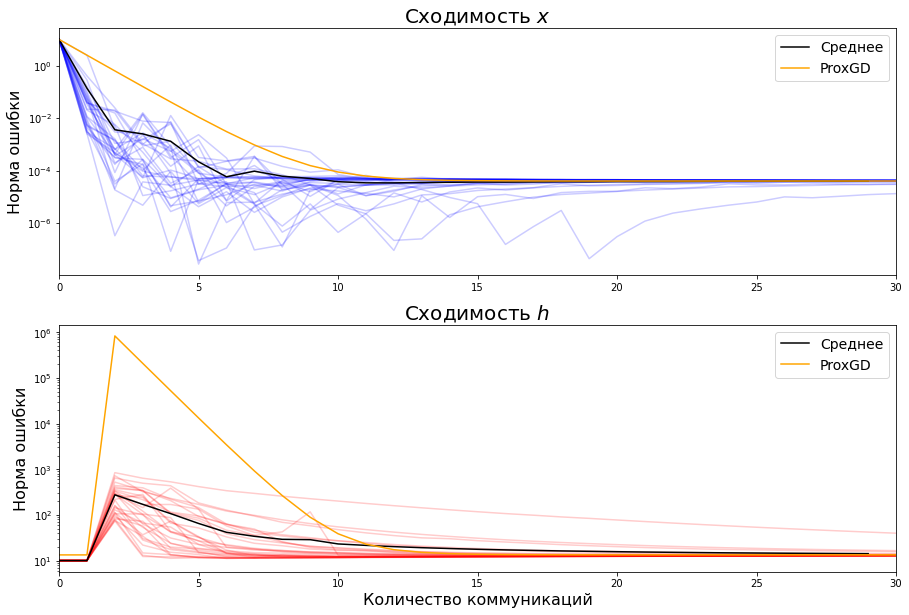
\includegraphics[scale=0.3]{ {./Scaffnew.png}}
\end{frame}

\begin{frame}{Сходимость Scaffnew при разных значениях $p$}
     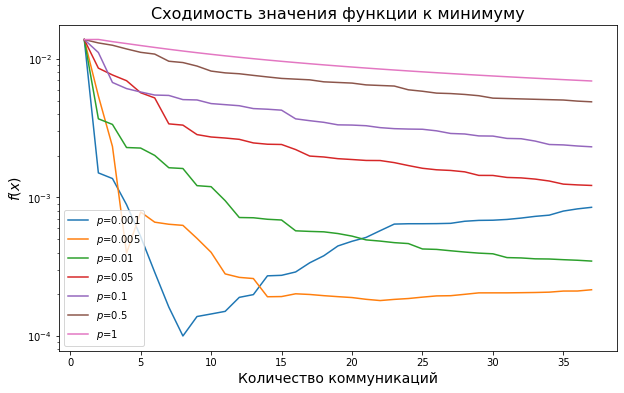
\includegraphics[scale=0.45]{ {./ScaffnewFunc.png}}
\end{frame}

\begin{frame}{Сходимость Scaffnew при разных значениях $p$}
     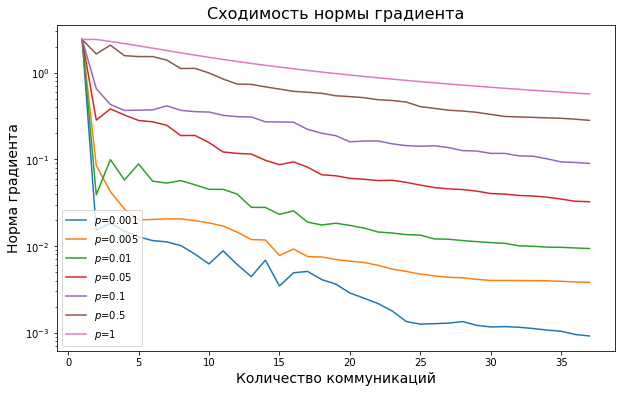
\includegraphics[scale=0.45]{ {./ScaffnewDifferentPs.png}}
\end{frame}

\begin{frame}{Обобщения и улучшения Scaffnew}
\begin{itemize}
    \item \textbf{Стохастический градиент}: в исходном Scaffnew $g$ было градиентом, вместо этого можно использовать несмещенные оценки градиента
    \item \textbf{Децентрализованное обучение}: Пусть дана \textit{матрица весов} $W$ - симметричная, положительно полуопределенная, с суммой элементов по каждой строке и каждому столбцу, равной 1. Можно рассмотреть задачу, когда в каждом раунде коммуникации в $i$-ой ноде оказывается взвешенное среднее $\sum\limits_{j=1}^n W_{i_j} x_j$, причем коммуникация происходит только для тех пар $i,\ j$, для которых $W_{i_j} \ne 0$. 
\end{itemize}
\end{frame}

\end{document}